\documentclass{article}

\usepackage[czech]{babel}
\usepackage[T1]{fontenc}
\usepackage[utf8]{inputenc}
\usepackage{amsmath,amsfonts,mathtools,multicol, url, booktabs}
\usepackage[a6paper, margin=20pt, landscape]{geometry}
\usepackage{graphicx, xcolor, tikz}
\usepackage{wrapfig, enumerate}
\parskip 10pt
\everymath{\displaystyle}
\parindent 0 pt


\def\zlomek{0.45}

\let\rho\varrho

\def\nic{}


\newcommand\obrazek[2][pixabay.com]{
  \clearpage
  \def\test{#1}
\begin{wrapfigure}{R}{\zlomek\linewidth}
  \begin{minipage}{1.0\linewidth}\parskip 0 pt
  \includegraphics[width=\linewidth]{#2}

  \vspace*{-10pt}
  \ifx\test\nic\else
  \null\hfill{\color{gray}\footnotesize Zdroj: #1}
  \fi

  \mezera
  \end{minipage}
\end{wrapfigure}
}

\let\oldtextbf\textbf
\def\textbf#1{%\newpage
  \oldtextbf{\color{red} #1}}

\def\mezera{\vspace*{10pt}}

\def\stranka{\newpage}


\begin{document}

\rightskip 0 pt plus 1 em
\title{Cvičení Matematika LDF, bak. 1. ročník}
\date{9. května 2019}

\maketitle

Řešení budou zveřejněna na webu předmětu
\url{http://user.mendelu.cz/marik/mt}.  

\def\div{\mathop{\mathrm{div}}}

\newpage

\textbf{Příklad 1.}
\begin{enumerate}[(i)]
\item Rovnici vedení tepla
\begin{equation*}
  \rho c \frac{\partial T}{\partial t}=\div (D\nabla T)
\end{equation*}
ve dvou dimenzích (pro plošný materiál) rozepište do složek v
kartézských souřadnicích. Uvažujte co nejobecnější případ
(nehomogenní, anizotropní).
\item 
Poté upravte rovnici z předchozího bodu pro jednu dimenzi (tyčový materiál).
\item 
Poté upravte rovnici z prvního bodu pro ortotropní materiál orientovaný tak, že
souřadné osy odpovídají vlastním směrům difuzní matice a koeficienty
difuzní matice nezávisí na prostorových souřadnicích (materiál je
homogenní).
\end{enumerate}
\newpage

\textbf{Příklad 2.} Stěnu oddělující dvě prostředí rozdílné teploty
můžeme modelovat jako tyč (velmi krátkou a tlustou, ale
jednorozměrnou), u které udržujeme konce na konstantních
teplotách. Ukažte, že ze stacionární rovnice vedení tepla plyne, že v
homogenním prostředí se teplota mění lineárně.

\newpage
\textbf{Příklad 3.} Budeme studovat rozložení teploty v dutém válci, u
kterého udržujeme na dvou rozdílných konstantních teplotách vnitřní a
vnější stěnu. Ukažte, že teplota se nemění lineárně.

\textbf{Návod:} Pro tyto případy je vhodné mít teplotu zapsánu nikoliv pomocí kartézských souřadnic, ale jako funkci vzdálenosti $r$ od počátku. 
Podle Wikipedie je
\begin{equation*}
  \frac{\partial^2 T}{\partial x^2}+  \frac{\partial^2 T}{\partial y^2}
    =
    \frac 1r \frac{\partial}{\partial r}\left(r\frac{\partial T}{\partial r}\right)+\frac 1{r^2}\frac{\partial ^2 T}{\partial \varphi^2},   
  \end{equation*}
  kde $r$ a $\varphi$ jsou polární souřadnice, vzdálenost od osy válce a odchylka od kladného směru osy $x$.

  
  \newpage

\textbf{Příklad 4.}
  Ukažte, že operátor divergence je možné psát ve tvaru
  \begin{equation*}
    \nabla \cdot \vec F,
  \end{equation*}
  kde $\vec F$ je vektorové pole, tečka značí skalární součin vektorů, pseudovektor $\nabla$ je definován vztahem
  \begin{equation*}
    \nabla =\left(\frac{\partial }{\partial x}, \frac{\partial }{\partial y}, \frac{\partial }{\partial z} \right)
  \end{equation*}
  a pseudosoučin výrazů $\frac{\partial}{\partial x}$ a $u$, tj výraz $\frac{\partial}{\partial x} u$ chápeme
  jako parciální derivaci.


  \newpage

  \let\overbar\overline
  \textbf{Příklad 5.}  V publikaci \textit{Berner et al, POD and Galerkin-based reduction of a wood chip drying model, IFAC PapersOnLine 50-1 (2017) 6619--6623}
  je studován model teplotního pole $T(y,t)$ a vlhkosti $x(y,t)$ v následujícím tvaru.

{\centering
  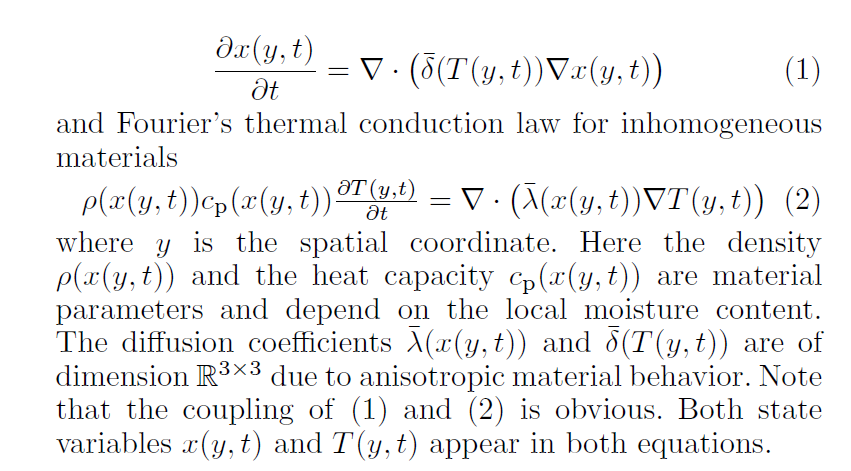
\includegraphics[width=0.7\linewidth]{berner.png}

  }

  
  Okomentujte rovnici a její jednotlivé členy. Jsou to difuzní rovnice, jak jsme se s nimi seznámili na přednášce? Je zde něco navíc? Chybí některý člen? Je možné něco říci o~předpokladech implicitně obsažených v takovéto konkrétní formulaci rovnic?
%   \begin{equation*}
%     \frac{\partial x(y,t)}{\partial t}=\nabla \cdot \Bigl(
% \overbar\delta (T(y,t))\nabla x(y,t)
%     \Bigr)
%   \end{equation*}
%   a
%   \begin{equation*}
%     \rho(x(y,t))c_p(x(y,t))\frac{\partial T(y,t)}{\partial t}
%     =\nabla\cdot \Bigl(\overbar \lambda(x(y,t))\nabla T(y,t)\Bigr).
%   \end{equation*}
%   Veličina $y$ je prostorová souřadnice, difuzní koeficienty $\overbar \lambda$ a $\overbar \delta$ jsou $3\times 3$ matice.  Jedná se o rovnice vedení
%   tepla, jak jsme si je představovali na přednášce? Jaká je
%   interpretace jednotlivých členů? Jaký mají zápis v~námi používané notaci?


  \newpage
    \textbf{Příklad 6.} 
\textit{  Gasparina et al, An adaptive simulation of nonlinear heat and
  moisture transfer as a boundary value problem, International Journal
  of Thermal Sciences 133 (2018) 120--139,} studují úlohu dle obrázku. Okomentujte rovnici a její jednotlivé členy.

{\centering
  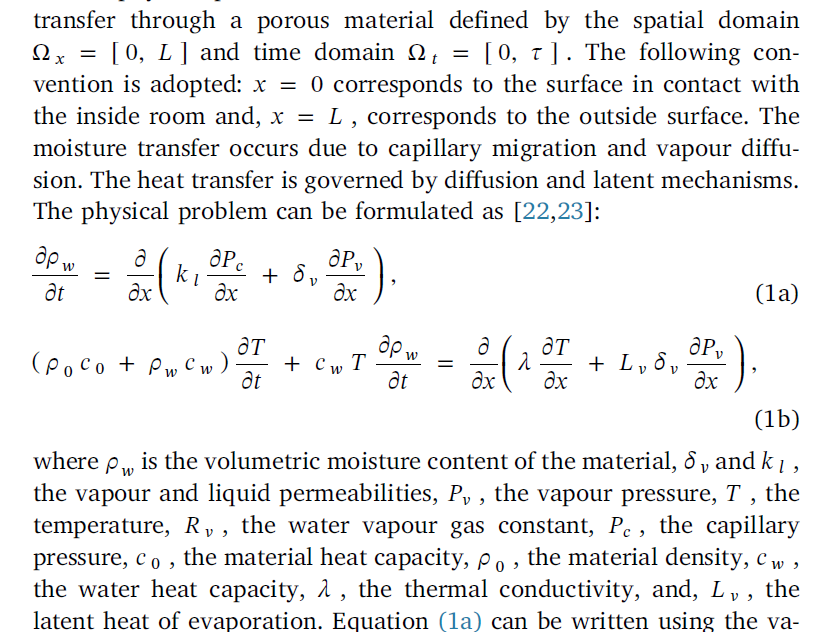
\includegraphics[width=0.7\linewidth]{gasparina.png}

  }

  \newpage \textbf{Příklad 7.}
\textit{Zhang et al, Simulation and validation of heat transfer during wood heat treatment
process, Results in Physics 7 (2017) 3806--3812,} studují úlohu dle obrázku. Okomentujte rovnici a její jednotlivé členy.

{\centering
  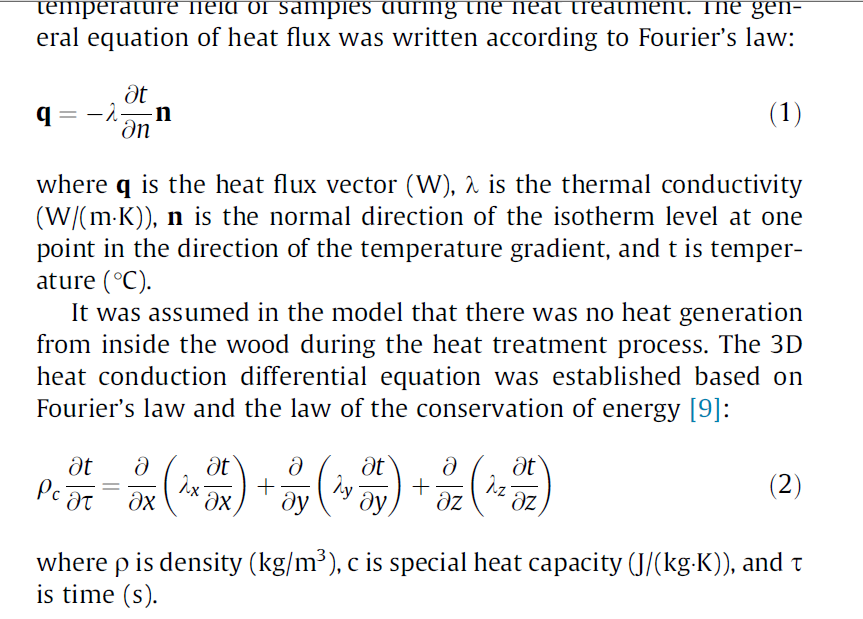
\includegraphics[width=0.7\linewidth]{zhang.png}

  }
  \newpage \textbf{Příklad 8.}
  \textit{Zhengbin He et al, Simulation of moisture transfer during wood vacuum drying, Results in Physics 12 (2019) 1299--1303,} studují úlohu dle obrázku. Okomentujte rovnici a její jednotlivé členy.

{  \centering
  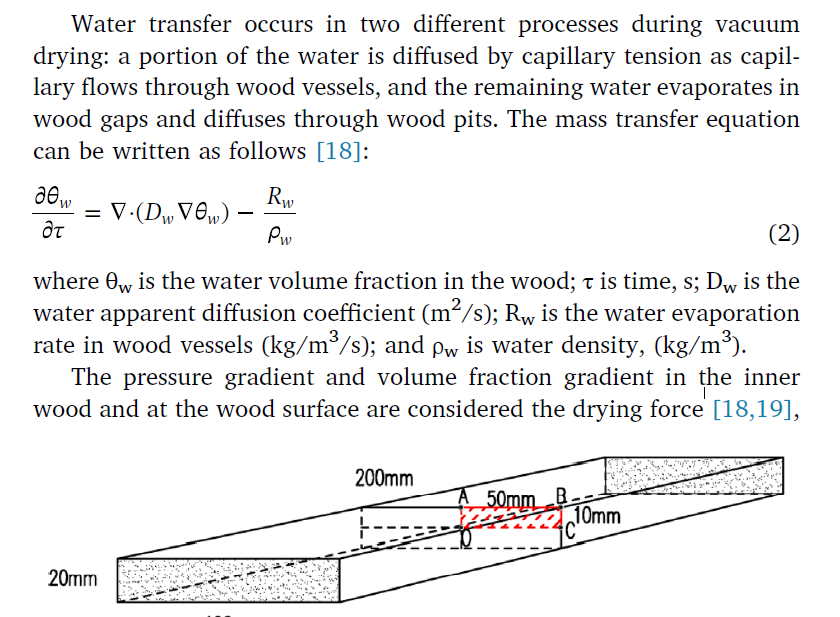
\includegraphics[width=0.7\linewidth]{he.png}

  }
\end{document}

